%%%%%%%%%%%%%%%%%%%%%%%%
%
% $Autor: Hemanth Jadiswami Prabhakaran $
% $Datum: 2026-09-13 $
% $Pfad: GitHub/MBIDA_Thesis/report/Contents/General/en/09EvaluationValidationConclusion.tex $
% $Version: 1 $
%
% $Project: MBIDA Thesis $
%
%%%%%%%%%%%%%%%%%%%%%%%%

\chapter{Evaluation -- Validation -- Conclusion}
\label{chap:evaluation}

This chapter reports the accuracy results the design decisions of Chapter~\ref{chap:methodology} and the implementation of Chapter~\ref{chap:appDevelopment} were built toward: sMAPE broken out by hierarchy level (Section~\ref{sec:accuracyByLevel}) and by business volume segment (Section~\ref{sec:accuracyByVolume}), together with four patterns that emerge from those two slices -- the Bottom-Up surprise, the high-volume baseline surprise, the Top-Down advantage on high-volume series, and the long-tail reversal. Section~\ref{sec:testingValidationResults} reports results against the testing protocol defined in Section~\ref{sec:testingValidation}. Sections~\ref{sec:answeringSQs}--\ref{sec:conclusionFutureWork} answer the sub-questions and the primary research question set out in Chapter~\ref{chap:introduction}, draw out practical recommendations for business forecasting practice, and revisit the limitations flagged in Section~\ref{sec:designLimitations}. Section~\ref{sec:monitoringOutlook} closes with a monitoring and operationalisation outlook for the dashboard introduced in Chapter~\ref{chap:appDeployment}. All figures below are computed on the test period only, at the point where actual outcomes are known and were withheld from model fitting (Section~\ref{sec:timeWindows}). These sMAPE figures are not directly comparable to the M5 competition's own official leaderboard rankings, which score submissions on price-weighted RMSSE (WRMSSE) rather than sMAPE -- a deliberate choice, not an oversight (Section~\ref{sec:smape}).

\section{Accuracy by Hierarchy Level}
\label{sec:accuracyByLevel}

Table~\ref{table:baseByLevel} reports sMAPE for the three unreconciled base models at each of the six hierarchy levels. Two patterns hold across all three models: accuracy degrades monotonically from Total down to Item, and the degradation is not gradual -- it is largest by far in the final step, from Department to Item. HistoricAverage's error roughly triples between these two levels (13.07\% to 40.91\%), and ETS's and Theta's error roughly quintuples. This mirrors the intermittency pattern established in Section~\ref{sec:intermittentDemand} and quantified in Section~\ref{sec:dataPreparation}: item-level series are sparse and irregular in a way that state- and store-level totals, smoothed by aggregation across many items, are not.

\begin{table}[htbp]
	\centering
	\caption{sMAPE (\%) by hierarchy level, base forecasts, test period.}
	\label{table:baseByLevel}
	\begin{tabular}{
			l
			S[table-format=2.2]
			S[table-format=2.2]
			S[table-format=2.2]
		}
		\toprule
		\textbf{Level} & {\textbf{Historic Average}} & {\textbf{ETS}} & {\textbf{Theta}} \\
		\midrule
		Total      &  6.58 &  5.53 &  4.24 \\
		State      &  6.85 &  4.88 &  4.32 \\
		Store      &  8.19 &  5.95 &  5.35 \\
		Category   & 11.32 &  7.31 &  6.73 \\
		Department & 13.07 &  7.88 &  8.26 \\
		Item       & 40.91 & 37.72 & 36.32 \\
		\bottomrule
	\end{tabular}
\end{table}

Between models, Theta is the most accurate base forecaster at every level except Department, where ETS is marginally ahead (7.88\% vs. 8.26\%); HistoricAverage is the least accurate base model at every level, although its gap narrows in relative terms at Item (40.91\% against Theta's 36.32\%), where intermittency dominates and seasonality is harder to exploit. This is consistent with the seasonal pattern established in Section~\ref{sec:seasonLength}: since HistoricAverage cannot represent the annual seasonality that \texttt{season\_length=12} lets ETS and Theta exploit, it is structurally disadvantaged wherever seasonality is present, and most clearly so at the smoother aggregate levels.

Reconciliation changes this picture substantially for ETS and Theta, and barely at all for HistoricAverage. Table~\ref{table:recByLevel} reports reconciled sMAPE for ETS and Theta under all three reconciliation methods (HistoricAverage is omitted here because, being already linear and therefore already coherent, Bottom-Up and Top-Down leave its values unchanged to two decimal places at every level, as Section~\ref{sec:testingValidationResults}'s coherence check confirms; MinTrace does the same on every level above Item, and only at Item does it raise the error from 40.91\% to 41.76\% -- see Table~\ref{table:smapeLevelHistavg} in the appendix).

\begin{table}[htbp]
	\centering
	\caption{Reconciled sMAPE (\%) by hierarchy level, ETS and Theta, test period.}
	\label{table:recByLevel}
	\begin{tabular}{ll S[table-format=2.2] S[table-format=2.2] S[table-format=2.2]}
		\toprule
		\textbf{Base model} & \textbf{Level} & {\textbf{Bottom-Up}} & {\textbf{MinTrace}} & {\textbf{Top-Down}} \\
		\midrule
		ETS   & Total      &  3.94 &  5.19 &  5.53 \\
		& State      &  3.97 &  5.11 &  5.88 \\
		& Store      &  4.77 &  5.58 &  7.60 \\
		& Category   &  6.22 &  7.19 & 10.63 \\
		& Department &  7.91 &  8.00 & 12.38 \\
		& Item       & 37.72 & 40.62 & 40.74 \\
		\addlinespace
		Theta & Total      &  3.78 &  4.36 &  4.24 \\
		& State      &  3.76 &  4.36 &  4.77 \\
		& Store      &  4.86 &  5.25 &  6.97 \\
		& Category   &  6.18 &  6.52 &  9.75 \\
		& Department &  7.60 &  7.98 & 11.49 \\
		& Item       & 36.32 & 39.24 & 40.54 \\
		\bottomrule
	\end{tabular}
\end{table}

\section{The Bottom-Up Surprise}
\label{sec:bottomUpSurprise}

Table~\ref{table:recByLevel} shows a largely consistent ranking at every level above Item, for both base models: Bottom-Up is the most accurate reconciler, MinTrace is usually second, and Top-Down is usually the least accurate. The one exception is Theta at the Total level, where Top-Down (4.24\%) edges out MinTrace (4.36\%) -- unsurprisingly, since Top-Down reproduces the base forecast at the root, and Theta's base Total forecast is already the most accurate of all base forecasts at that level. At the Total level, for example, ETS's Bottom-Up forecast reaches 3.94\% sMAPE against MinTrace's 5.19\% and the unreconciled base forecast's own 5.53\% -- MinTrace's theoretically motivated cross-level adjustment leaves the series worse off than simply summing the item-level forecasts upward. The gap between Bottom-Up and MinTrace is largest at the top of the hierarchy and narrows moving down it: for ETS it shrinks from 1.25 percentage points at Total to 1.14 at State, 0.81 at Store, 0.97 at Category and only 0.09 at Department, while for Theta it stays between roughly 0.35 and 0.6 points throughout. At Item the gap reopens (2.9 points for both models), because Bottom-Up is there definitionally identical to the unreconciled item-level forecast, while MinTrace's non-negative adjustment moves many item-level forecasts away from it.

This runs against the usual framing of MinTrace as the theoretically optimal reconciler, in the specific sense proved in Section~\ref{subsec:minTrace} \cite{Wickramasuriya:2019}, so it is worth setting out two candidate explanations rather than treating MinTrace's superiority as a given. First, the \texttt{wls\_struct} weighting scheme used here -- $W = \operatorname{diag}(S\mathbf{1})$, as derived in Section~\ref{subsec:minTrace} and adopted here for the reasons given in Section~\ref{sec:designLimitations} -- scales each node purely by how many bottom-level series sum into it, not by an estimate of that node's own forecast-error variance -- a coarser signal than the shrinkage-based covariance estimator a full MinTrace implementation would use, and one that gives the method less information to act on than its reputation assumes. Second, the upper levels of this hierarchy are already comparatively stable and non-intermittent, as established in Section~\ref{sec:intermittentDemand} and Section~\ref{sec:dataPreparation}: with little genuine incoherence left for Bottom-Up's plain summation to correct, MinTrace's cross-level adjustment has more room to introduce noise than to remove it. Both explanations point the same way -- toward \texttt{wls\_struct} specifically, rather than reconciliation in general, being the weaker link -- which is why Section~\ref{sec:designLimitations} flags a shrinkage-based MinTrace variant as future work rather than concluding that Bottom-Up is simply the better method.

\section{Accuracy by Volume Segment}
\label{sec:accuracyByVolume}

The volume-percentile framework defined in Section~\ref{sec:volumeFramework} ranks the 30,240 bottom-level (item-store) series by training-period sales volume and buckets them by cumulative share of that volume. Figure~\ref{fig:paretoCurve} shows this concentration directly: plotting the cumulative share of training-period volume against the cumulative share of series, ranked biggest seller first, produces a curve far steeper than the perfectly-even diagonal it is plotted against. Table~\ref{table:volumeBuckets} restates the same concentration numerically: the top 5\% of training volume comes from only 29 series (0.10\% of all series), and even the top 80\% of volume comes from just 8,155 series (26.97\% of all series) -- the remaining roughly three-quarters of all series account for only the last fifth of total volume.

\begin{figure}[h]
	\centering
	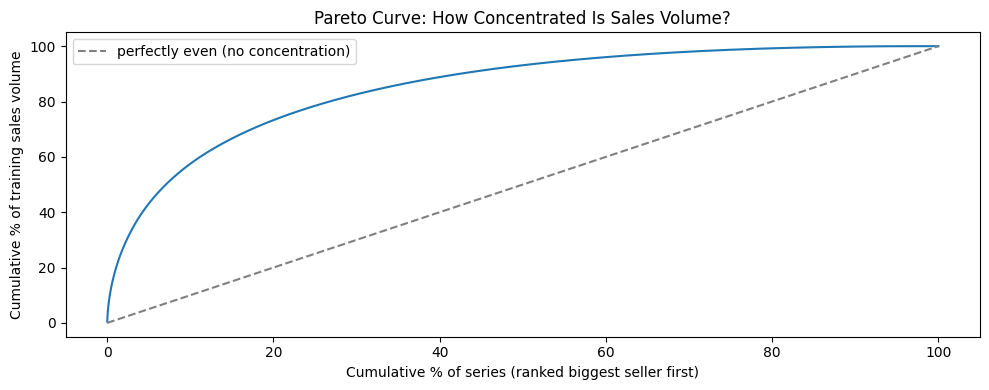
\includegraphics[width=0.8\linewidth]{Images/09EvaluationValidationConclusion/paretoCurve}
	\caption{Pareto curve of training-period sales volume: cumulative share of volume against cumulative share of bottom-level series, ranked from the largest seller. Source: \texttt{01\_eda.ipynb}.}\label{fig:paretoCurve}
\end{figure}

\begin{table}[htbp]
	\centering
	\caption{Volume-bucket sizes, ranked on training-period volume.}
	\label{table:volumeBuckets}
	\begin{tabular}{
			S[table-format=3.0]
			S[table-format=5.0, group-separator={,}]
			S[table-format=3.2]
		}
		\toprule
		{\textbf{Top \% of volume}} & {\textbf{Series in bucket}} & {\textbf{\% of all 30,240 series}} \\
		\midrule
		5 &    29 &   0.10 \\
		10 &    94 &   0.31 \\
		20 &   326 &   1.08 \\
		50 &  2151 &   7.11 \\
		80 &  8155 &  26.97 \\
		100 & 30240 & 100.00 \\
		\bottomrule
	\end{tabular}
\end{table}

Table~\ref{table:volumeBaseAccuracy} reports base-forecast sMAPE within each bucket. Because these buckets are cumulative and nested -- the top 10\% bucket contains the top 5\% bucket, and so on -- the top 100\% row is identical to the Item row of Table~\ref{table:baseByLevel}, confirmed to six decimal places in the pipeline's own output (a consequence of the evaluation grid being perfectly balanced, since every series contributes exactly the same 12 zero-filled test-period rows).

\begin{table}[htbp]
	\centering
	\caption{sMAPE (\%) by volume segment, base forecasts, test period.}
	\label{table:volumeBaseAccuracy}
	\begin{tabular}{
			S[table-format=3.0]
			S[table-format=2.2]
			S[table-format=2.2]
			S[table-format=2.2]
		}
		\toprule
		{\textbf{Top \% of volume}} & {\textbf{Historic Average}} & {\textbf{ETS}} & {\textbf{Theta}} \\
		\midrule
		5 & 16.61 & 22.97 & 22.97 \\
		10 & 22.51 & 29.88 & 30.41 \\
		20 & 27.89 & 33.43 & 32.79 \\
		50 & 28.88 & 31.93 & 31.04 \\
		80 & 29.68 & 31.84 & 31.10 \\
		100 & 40.91 & 37.72 & 36.32 \\
		\bottomrule
	\end{tabular}
\end{table}

\section{The High-Volume Baseline Surprise}
\label{sec:highVolumeBaselineSurprise}

Table~\ref{table:volumeBaseAccuracy} shows HistoricAverage as the most accurate base model in every bucket up to and including the top 80\% of volume, and by a wide margin in the smallest, highest-volume buckets: at the top 5\% of volume, HistoricAverage reaches 16.61\% sMAPE against ETS's and Theta's 22.97\%, roughly six percentage points better. Only at the top 100\% bucket -- once the long tail of low-volume, high-intermittency series is folded in -- does this ranking invert, with Theta (36.32\%) and ETS (37.72\%) overtaking HistoricAverage (40.91\%).

This is the opposite of what the seasonal argument in Section~\ref{sec:seasonLength} might suggest on its own: ETS and Theta were configured specifically to exploit the annual seasonality visible in aggregate sales, yet on the series that carry the most sales volume, the flat, no-seasonality HistoricAverage baseline wins. This is not an isolated anomaly; it echoes one of the most robust findings in the forecasting literature, that simple extrapolative methods frequently match or beat statistically more sophisticated ones on real data \cite{MakridakisHibon:2000}. A plausible reading is that individual high-volume series still carry enough month-to-month idiosyncrasy -- promotions, calendar effects, one-off spikes -- that a seasonal decomposition fitted to only four years of monthly training data (Section~\ref{sec:dataset}) picks up noise as if it were a repeating pattern, whereas HistoricAverage's flat mean is not exposed to that risk. Whatever the mechanism, the practical implication carried into Section~\ref{sec:practicalRecommendations} is direct: "more sophisticated" is not a safe default assumption for the series a business actually cares most about.

\section{The Top-Down Advantage on High-Volume Series}
\label{sec:topDownAdvantage}

Reconciliation interacts with volume segment as strongly as it interacts with hierarchy level. Table~\ref{table:volumeReconciled} isolates Bottom-Up and Top-Down for ETS and Theta across the same volume buckets as Table~\ref{table:volumeBaseAccuracy} (MinTrace tracks Bottom-Up closely up to the top 80\% bucket and is omitted for readability; its full figures, including the larger gap at the top 100\% bucket, are given in Tables~\ref{table:smapeVolumeEts} and~\ref{table:smapeVolumeTheta} in the appendix).

\begin{table}[htbp]
	\centering
	\setlength{\tabcolsep}{5pt}
	\caption{Reconciled sMAPE (\%) by volume segment: Bottom-Up vs.\ Top-Down.}
	\label{table:volumeReconciled}
	\begin{tabular}{
			S[table-format=3.0]
			S[table-format=2.2]
			S[table-format=2.2]
			S[table-format=2.2]
			S[table-format=2.2]
		}
		\toprule
		& \multicolumn{2}{c}{\textbf{ETS}} & \multicolumn{2}{c}{\textbf{Theta}} \\
		\cmidrule(lr){2-3} \cmidrule(lr){4-5}
		{\makecell{\textbf{Top \% of}\\\textbf{volume}}} & 
		{\makecell{\textbf{Bottom-}\\\textbf{Up}}} & 
		{\makecell{\textbf{Top-}\\\textbf{Down}}} & 
		{\makecell{\textbf{Bottom-}\\\textbf{Up}}} & 
		{\makecell{\textbf{Top-}\\\textbf{Down}}} \\
		\midrule
		5 & 22.97 & 16.98 & 22.97 & 17.47 \\
		10 & 29.88 & 22.91 & 30.41 & 23.42 \\
		20 & 33.43 & 28.14 & 32.79 & 28.48 \\
		50 & 31.93 & 28.99 & 31.04 & 29.16 \\
		80 & 31.84 & 29.69 & 31.10 & 29.73 \\
		100 & 37.72 & 40.74 & 36.32 & 40.54 \\
		\bottomrule
	\end{tabular}
\end{table}

Figure~\ref{fig:volumeReconciledChart} plots the same numbers directly: Top-Down (dashed) sits clearly below Bottom-Up (solid) across the narrow, high-volume buckets, then crosses above it by the top 100\% bucket -- the reversal described in Section~\ref{sec:longTailReversal} is visible here as the two line styles trading places, rather than only as a change of sign in a table of numbers.

\begin{figure}[h]
	\centering
	\includegraphics[width=0.8\linewidth]{Images/09EvaluationValidationConclusion/volumeReconciledChart}
	\caption{Reconciled sMAPE by volume segment for ETS and Theta, Bottom-Up (solid) vs. Top-Down (dashed).}\label{fig:volumeReconciledChart}
\end{figure}

At the top 5\% of volume, Top-Down cuts ETS's sMAPE from 22.97\% (Bottom-Up) to 16.98\%, and Theta's from 22.97\% to 17.47\% -- close to HistoricAverage's own 16.61\% in Table~\ref{table:volumeBaseAccuracy}, and clearly the best reconciled result in this segment for either model. The advantage persists, though it narrows, through the top 10\%, 20\%, 50\%, and 80\% buckets. This is the inverse of Section~\ref{sec:bottomUpSurprise}'s finding at the hierarchy-level view: there, Top-Down was almost uniformly the weakest reconciler; here, restricted to the series that carry the most volume, it is the strongest. Top-Down's proportional redistribution of the Total forecast by historical volume share -- the proportions vector $p$ formalised in Section~\ref{subsec:topDown} -- is, by construction, most reliable precisely where a series' historical share of volume is itself a stable, representative quantity -- true of high-volume series, and decreasingly true as the buckets widen to include smaller, more erratic ones.

\section{The Long-Tail Reversal}
\label{sec:longTailReversal}

The advantage identified in Section~\ref{sec:topDownAdvantage} does not merely shrink as the volume buckets widen -- it reverses. At the top 100\% bucket in Table~\ref{table:volumeReconciled}, Top-Down is the \emph{worst} of the two reconcilers for both base models (ETS: 40.74\% vs. Bottom-Up's 37.72\%; Theta: 40.54\% vs. 36.32\%), even though it was the best at every narrower, higher-volume bucket. The reversal is driven by the same long tail identified in Section~\ref{sec:highVolumeBaselineSurprise}: the roughly three-quarters of series that carry only the last fifth of total volume (Table~\ref{table:volumeBuckets}) have volume shares too small and too erratic for Top-Down's proportional split to track, while Bottom-Up's item-level fits -- however imprecise individually -- are not tied to any assumption about historical share at all.

Read together with Section~\ref{sec:highVolumeBaselineSurprise}, this reversal marks out exactly where each method earns its keep: HistoricAverage and Top-Down are strongest on the small number of series that dominate training-period sales volume, while ETS and Theta under Bottom-Up reconciliation only pull ahead once the long tail is counted. The fairness note in Section~\ref{sec:fairnessNote} flags the consequence directly -- because the volume-percentile framework's headline comparisons foreground high-volume performance, they structurally under-weight exactly the segment, and exactly the models, this reversal shows to be worth measuring on their own terms.

\section{Testing \& Validation Results}
\label{sec:testingValidationResults}

Table~\ref{table:sanityChecks} reports results against the three checks specified in Section~\ref{sec:testingValidation}, together with the negative-forecast check that verifies the clipping decision motivated in Section~\ref{sec:clippingRationale}.

\begin{table}[htbp]
	\centering
	\small
	\caption{Testing and validation results, against the protocol defined in Section~\ref{sec:testingValidation}.}
	\label{table:sanityChecks}
	\begin{tabular}{@{} p{5.2cm} p{4.6cm} p{3.0cm} @{}}
		\toprule
		\textbf{Check} & \textbf{Result} & \textbf{Expected} \\
		\midrule
		Coherence (\textit{HistoricAverage} vs.\ Bottom-Up) & max diff 0.146244 & $\approx 0$ \\
		\addlinespace
		Top-Down root invariance (ETS, Total level) & max diff 0.000000 & $\approx 0$ \\
		\addlinespace
		Fallback rate (ETS)   & 699 of 30,354 series (2.30\%) & monitored \\
		Fallback rate (Theta) & 699 of 30,354 series (2.30\%) & monitored \\
		\addlinespace
		Negative-forecast check (all columns, post-clipping) & 0 negatives everywhere & 0 \\
		\bottomrule
	\end{tabular}
\end{table}

All three checks pass. The coherence check's max difference of 0.146244, rather than an exact 0, reflects ordinary floating-point accumulation across the reconciliation pipeline and is negligible against sMAPE values reported in whole percentage points; the Top-Down root check is exact, confirming the single "Total" root added in Section~\ref{sec:totalRoot} behaves as required. ETS and Theta fall back to HistoricAverage on identically 699 of 30,354 series (2.30\%) -- the same series in both cases, since both models' fitting routines fail under the same conditions of short or irregular history. This 2.30\% figure is not itself a pass/fail criterion but a baseline worth carrying into Section~\ref{sec:monitoringOutlook}: a materially higher rate on a future run of this pipeline would be a signal that the item universe or data quality has shifted. The negative-forecast check confirms that clipping base forecasts before reconciliation (Section~\ref{sec:clippingRationale}) succeeded: no base or reconciled column contains a negative value, where before clipping 2,300 ETS and 16,345 Theta test-period values had been negative.

\section{Answering SQ1--SQ3 and the Primary Research Question}
\label{sec:answeringSQs}

\textbf{SQ1 -- Do Bottom-Up, Top-Down, and MinTrace differ in accuracy patterns across hierarchy levels?} Yes, and the difference is not a fixed ranking but one that depends on where in the hierarchy the question is asked. Section~\ref{sec:bottomUpSurprise} shows Bottom-Up ahead of MinTrace and Top-Down at every level from Total to Department; Top-Down is the weakest of the three at the hierarchy-level view at every level except Theta's Total, where it simply reproduces Theta's already accurate base forecast. The three methods are not interchangeable, and no single one of them is the safe default across the whole hierarchy.

\textbf{SQ2 -- Does the choice of base model affect reconciliation performance across the hierarchy?} Yes, substantially, but not because reconciliation reacts differently to each base model's forecasts as such -- rather, because HistoricAverage is already linear and therefore already coherent (Section~\ref{sec:testingValidationResults}), reconciliation changes almost nothing for it, while ETS's and Theta's forecasts are genuinely incoherent across levels and see multi-percentage-point swings under different reconcilers (Table~\ref{table:recByLevel}). The base model determines not just the starting accuracy but whether reconciliation has any real work to do.

\textbf{SQ3 -- As the evaluation widens from the highest-volume series outward to the full population, how does the gap between methods change?} It does not merely narrow -- it inverts, twice over. Sections~\ref{sec:highVolumeBaselineSurprise} and~\ref{sec:topDownAdvantage} show HistoricAverage and Top-Down leading on the narrowest, highest-volume buckets; Section~\ref{sec:longTailReversal} shows Theta, ETS, and Bottom-Up overtaking them once the long tail is included. Which combination looks best is therefore inseparable from which slice of the business the question is being asked about.

\textbf{Primary research question -- how do foundational hierarchical forecasting methods perform across volume segments, and what practical insights follow?} No single base-model/reconciliation combination dominates across both dimensions examined in this thesis. Performance is segment-dependent along business volume (Sections~\ref{sec:highVolumeBaselineSurprise}--\ref{sec:longTailReversal}) and level-dependent along the hierarchy (Sections~\ref{sec:accuracyByLevel}--\ref{sec:bottomUpSurprise}), and the two dependencies do not point the same direction: the combination that performs best on high-volume series (HistoricAverage or Top-Down-reconciled ETS/Theta) is not the combination that performs best once the long tail is counted (Bottom-Up-reconciled ETS/Theta). Practical insights follow directly in Section~\ref{sec:practicalRecommendations}.

\section{Practical Recommendations for Business Forecasting Practice}
\label{sec:practicalRecommendations}

Three recommendations follow directly from the results above, aimed at a practitioner choosing a forecasting setup for a similar retail hierarchy rather than at further model development.

First, match the method to the business question rather than adopting one combination hierarchy-wide. Where the decision concerns the small number of high-volume item-store series -- the "A" items of an ABC classification, whose replenishment and stock levels carry the most business weight -- HistoricAverage or a Top-Down-reconciled base model is both simpler to explain and more accurate than the alternatives (Sections~\ref{sec:highVolumeBaselineSurprise}--\ref{sec:topDownAdvantage}). This finding concerns individual high-volume series, not the aggregate levels of the hierarchy: for headline reporting and top-line planning at the Total, State or Store level, Bottom-Up remains the more accurate reconciler and Top-Down generally the least accurate (Section~\ref{sec:bottomUpSurprise}). Where the audience is item-level replenishment or long-tail inventory decisions, Bottom-Up-reconciled ETS or Theta is the better-performing choice (Section~\ref{sec:longTailReversal}), and this is exactly the segment the fairness note in Section~\ref{sec:fairnessNote} warns is otherwise under-weighted by volume-percentile evaluation alone.

Second, do not treat MinTrace's theoretical optimality as a guarantee of practical superiority without checking the specific variant in use. The \texttt{wls\_struct} weighting evaluated here underperforms simple Bottom-Up summation at every hierarchy level above Item (Section~\ref{sec:bottomUpSurprise}); a shrinkage-based variant, flagged as future work in Section~\ref{sec:designLimitations}, would need to be checked on the same data before MinTrace could be recommended over Bottom-Up in this setting.

Third, do not assume a more sophisticated, seasonally aware model beats a naive baseline by default. HistoricAverage's advantage on high-volume series (Section~\ref{sec:highVolumeBaselineSurprise}) is large enough -- more than six percentage points in the top 5\% bucket -- that it should be treated as a genuine competitor rather than a mere reference point in any comparable evaluation.

\section{Conclusion and Future Work}
\label{sec:conclusionFutureWork}

This thesis set out to compare foundational hierarchical forecasting methods across hierarchy levels and business volume segments on retail demand data, and to draw out what those comparisons imply for practice. The empirical picture that emerges is one of segment-dependence rather than a single winning combination: Bottom-Up reconciliation outperforms MinTrace and Top-Down above the Item level; HistoricAverage and Top-Down outperform ETS, Theta, and Bottom-Up on high-volume series; and this ranking reverses once the long tail is included. Together these findings answer SQ1--SQ3 and the primary research question as set out in Section~\ref{sec:answeringSQs}.

The limitations set out in Section~\ref{sec:designLimitations} bound how far these conclusions generalise. Most directly, the \texttt{wls\_struct} MinTrace variant used throughout this thesis is not the only MinTrace variant available, and the Bottom-Up surprise reported in Section~\ref{sec:bottomUpSurprise} should be re-examined against a shrinkage-based covariance estimator before concluding that MinTrace itself, rather than this specific weighting choice, underperforms. The single-dataset scope of this thesis (Section~\ref{sec:dataset}) means these patterns are demonstrated on M5's retail hierarchy specifically, not established as general properties of hierarchical forecasting; and the monthly aggregation adopted in Section~\ref{sec:dailyToMonthly} trades away any intra-month granularity a business might separately need. Each of these is a natural next step rather than a gap in the study as scoped.

\section{Monitoring \& Operationalisation Outlook}
\label{sec:monitoringOutlook}

The dashboard described in Chapter~\ref{chap:appDeployment} currently serves forecasts for a live period with no ground truth to check them against (Section~\ref{sec:timeWindows}); as real sales data for that period becomes available, the same sMAPE evaluation used throughout this chapter could be re-run against it on a rolling basis, at both the hierarchy-level and volume-segment views, to confirm the patterns identified here persist rather than being artifacts of the single train/test split used in this thesis.

The 2.30\% fallback rate established in Section~\ref{sec:testingValidationResults} is a natural health metric to track over time: since it reflects how often ETS and Theta fail to fit and fall back to HistoricAverage, a sustained increase would indicate that the item universe, data quality, or model configuration needs attention before accuracy figures are trusted. Similarly, because Section~\ref{sec:longTailReversal} shows accuracy ranking to be volume-segment-dependent, any operational monitoring should track sMAPE separately by volume bucket rather than as a single hierarchy-wide average, since a stable overall figure could otherwise mask deterioration concentrated in one segment. Retraining cadence, drift detection thresholds, and extension of the comparison to a shrinkage-based MinTrace variant (Section~\ref{sec:conclusionFutureWork}) are the most direct next steps toward turning this thesis's one-off evaluation into an operational monitoring practice.